\section{Bloque 4}\label{sec:bloque_4}

\textbf{Convenios del bloque.} El estado marcado se escribe $w=x_{n-1}\dots x_0$, con $x_j$ en el qubit $q_j$ (convenio \emph{little-endian} de Qiskit), de modo que $|w\rangle$
es el elemento de índice $\mathrm{int}(w,2)$ del vector de estado. Para $n=3$ y $w=011$ se marca el estado $|3\rangle$.

El \textbf{oráculo de fase} $O|x\rangle=-|x\rangle$ si $x=w$ y $O|x\rangle=|x\rangle$ en otro caso se construye con una puerta $Z$ multicontrolada
($H\cdot\mathrm{MCX}\cdot H$ sobre el último qubit), rodeando con puertas $X$ los qubits en los que $w$ tiene un 0. El \textbf{operador de difusión}
$D=2|s\rangle\langle s|-I=H^{\otimes n}(2|0\rangle\langle0|-I)H^{\otimes n}$ se implementa con $H^{\otimes n}$, $X^{\otimes n}$, una $Z$ multicontrolada, de nuevo $X^{\otimes n}$ y $H^{\otimes n}$.
Este circuito produce en realidad $-D$ (la $Z$ multicontrolada es $I-2|1\dots1\rangle\langle1\dots1|$, y conjugada con $X^{\otimes n}$ y $H^{\otimes n}$ da $I-2|s\rangle\langle s|$), de modo que se le añade una fase global $\pi$ para que
coincida exactamente con $D$. El algoritmo completo aplica $H^{\otimes n}$ a $|0\rangle^{\otimes n}$, $k$ iteraciones de $G=D\cdot O$ y mide los $n$ qubits.

Para las predicciones se usa $P_k(w)=\sin^2((2k+1)\theta)$ con $\sin\theta=1/\sqrt{N}$. Se emplea \texttt{Statevector} (circuito sin medidas) para las amplitudes y
\texttt{AerSimulator} con 4096 disparos y semilla fija para los histogramas.

%--------------------------------------------------------------------
\subsection{Ejercicio 4.1. Aplicación del operador de difusión}
Para $n=3$ ($N=8$) se parte del estado que resulta de aplicar el oráculo que marca $|3\rangle=|011\rangle$ a la superposición uniforme $|s\rangle=H^{\otimes3}|000\rangle$,
$$|a\rangle=O|s\rangle=\sum_i a_i|i\rangle,\qquad a_i=\tfrac{1}{\sqrt8}\ \ (i\neq3),\qquad a_3=-\tfrac{1}{\sqrt8}.$$
El oráculo de fase correspondiente se muestra en la Figura~\ref{fig:bloque4_e4_1_oraculo}. Como $w=011$ solo tiene un 0 (en el bit de $q_2$), basta una puerta $X$ en $q_2$ antes y después de la $Z$ multicontrolada, que se construye como $H\cdot\mathrm{MCX}\cdot H$ sobre $q_2$.

\begin{figure}[h]
    \centering
    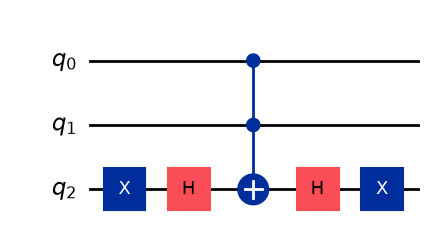
\includegraphics[width=0.6\textwidth]{imagenes/bloque4/e4_1_oraculo.png}
    \caption{Oráculo de fase $O_w$ que marca el estado $|3\rangle=|011\rangle$: $X$ en $q_2$, $Z$ multicontrolada ($H\cdot\mathrm{MCX}\cdot H$ sobre $q_2$) y de nuevo $X$ en $q_2$.}\label{fig:bloque4_e4_1_oraculo}
\end{figure}

\textbf{Cálculo a mano.} La difusión es una inversión respecto a la media, $b_i=2\bar a-a_i$. La media es
$$\bar a=\frac18\Big(7\cdot\frac{1}{\sqrt8}-\frac{1}{\sqrt8}\Big)=\frac{6}{8\sqrt8}=\frac{3}{4\sqrt8}\approx0{,}26517,$$
y por tanto
$$b_i=\frac{3}{2\sqrt8}-\frac{1}{\sqrt8}=\frac{1}{2\sqrt8}\approx0{,}17678\quad(i\neq3),\qquad
b_3=\frac{3}{2\sqrt8}+\frac{1}{\sqrt8}=\frac{5}{2\sqrt8}\approx0{,}88388.$$
La probabilidad de medir el estado marcado pasa de $a_3^2=1/8=0{,}125$ a $b_3^2=25/32\approx0{,}781$. Se comprueba que la suma de probabilidades es 1:
$7\cdot\frac{1}{32}+\frac{25}{32}=1$.

\textbf{Comprobación con el circuito.} El operador de difusión $D=2|s\rangle\langle s|-I=H^{\otimes n}(2|0\rangle\langle0|-I)H^{\otimes n}$ se implementa con el circuito de la Figura~\ref{fig:bloque4_e4_1_difusion}: $H^{\otimes3}$, $X^{\otimes3}$, $Z$ multicontrolada, $X^{\otimes3}$ y $H^{\otimes3}$. Este montaje produce en realidad $-D$, por lo que se le añade una fase global $\pi$ para que coincida exactamente con $D$.

\begin{figure}[h]
    \centering
    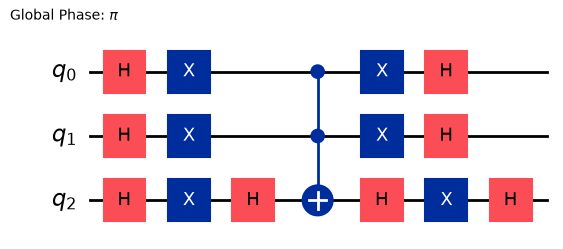
\includegraphics[width=0.6\textwidth]{imagenes/bloque4/e4_1_operado_difusion.png}
    \caption{Circuito del operador de difusión $D$ para $n=3$ (con fase global $\pi$).}\label{fig:bloque4_e4_1_difusion}
\end{figure}

Se verifica con \texttt{Statevector} que: (i) $O|s\rangle=|a\rangle$, (ii) la matriz del circuito
coincide con $2|s\rangle\langle s|-I$ y (iii) $D|a\rangle$ coincide con el vector $|b\rangle$ calculado a mano (Tabla~\ref{tab:bloque4_e4_1}).

\begin{table}[htbp]
    \centering
    \begin{tabular}{c|c|c|c|c}
    \hline
    $i$ & $|i\rangle$ & $a_i$ & $b_i$ (a mano) & $b_i$ (circuito) \\
    \hline
    0 & \texttt{000} &  0,35355 & 0,17678 & 0,17678 \\
    1 & \texttt{001} &  0,35355 & 0,17678 & 0,17678 \\
    2 & \texttt{010} &  0,35355 & 0,17678 & 0,17678 \\
    3 & \texttt{011} & $-0{,}35355$ & 0,88388 & 0,88388 \\
    4 & \texttt{100} &  0,35355 & 0,17678 & 0,17678 \\
    5 & \texttt{101} &  0,35355 & 0,17678 & 0,17678 \\
    6 & \texttt{110} &  0,35355 & 0,17678 & 0,17678 \\
    7 & \texttt{111} &  0,35355 & 0,17678 & 0,17678 \\
    \hline
    \end{tabular}
    \caption{Ejercicio 4.1: amplitudes antes ($a_i$) y después ($b_i$) de aplicar el operador de difusión.}\label{tab:bloque4_e4_1}
\end{table}

El circuito completo de una iteración, $H^{\otimes3}\to O\to D$, se muestra en la Figura~\ref{fig:bloque4_e4_1_completo}; su vector de estado final coincide con $|b\rangle$. La Figura~\ref{fig:bloque4_e4_1_efecto} muestra el efecto de la inversión respecto a la media.

\begin{figure}[h]
    \centering
    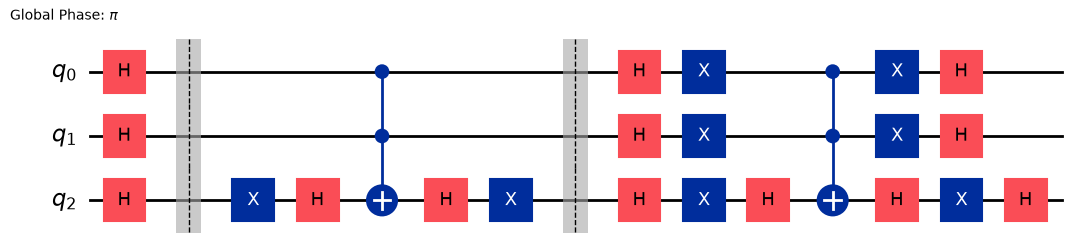
\includegraphics[width=\textwidth]{imagenes/bloque4/e4_1_circuito_completo.png}
    \caption{Circuito completo de una iteración de Grover para $N=8$ y $w=011$: preparación de $|s\rangle$, oráculo $O$ y operador de difusión $D$ (con fase global $\pi$).}\label{fig:bloque4_e4_1_completo}
\end{figure}

\begin{figure}[h]
    \centering
    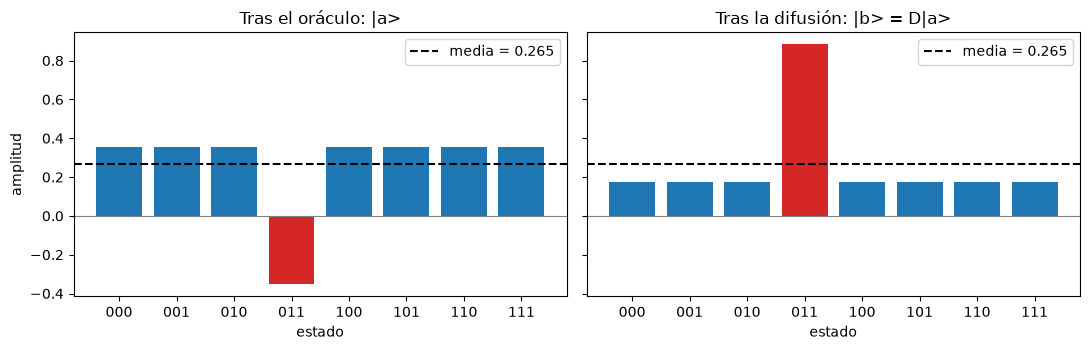
\includegraphics[width=\textwidth]{imagenes/bloque4/e4_1_efecto_difusion.png}
    \caption{Amplitudes tras el oráculo (izquierda) y tras el operador de difusión (derecha). La línea discontinua es la media de las amplitudes; el estado marcado, $|011\rangle$, está en rojo.}\label{fig:bloque4_e4_1_efecto}
\end{figure}

\textbf{Resultado.} El resultado simulado coincide con el calculado a mano. Tras el oráculo, la amplitud del estado marcado es negativa y queda muy por debajo de la media ($0{,}265$);
al invertir respecto a la media pasa de $-0{,}354$ a $+0{,}884$, mientras que las demás amplitudes disminuyen ligeramente, de $0{,}354$ a $0{,}177$. Así, una sola iteración aumenta la probabilidad del estado marcado de $0{,}125$ a $0{,}781$.

%--------------------------------------------------------------------
\subsection{Ejercicio 4.2. Número de iteraciones}
Para $N=8$ y un único estado marcado ($w=011$), $\theta=\arcsin(1/\sqrt8)=0{,}36137$ rad $=20{,}70^\circ$, y la probabilidad de éxito tras $k$ iteraciones es $P_k(w)=\sin^2((2k+1)\theta)$.
La Tabla~\ref{tab:bloque4_e4_2_pk} compara este valor con el obtenido en la simulación para $k=0,\dots,4$.

\begin{table}[htbp]
    \centering
    \begin{tabular}{c|c|c|c}
    \hline
    $k$ & $(2k+1)\theta$ (rad) & $P_k$ teórica & $P_k$ simulada \\
    \hline
    0 & 0,3614 & 0,1250 & 0,1313 \\
    1 & 1,0841 & 0,7813 & 0,7795 \\
    2 & 1,8068 & 0,9453 & 0,9475 \\
    3 & 2,5296 & 0,3301 & 0,3318 \\
    4 & 3,2523 & 0,0122 & 0,0115 \\
    \hline
    \end{tabular}
    \caption{Ejercicio 4.2: probabilidad de éxito de Grover para $N=8$ en función del número de iteraciones $k$.}\label{tab:bloque4_e4_2_pk}
\end{table}

El mínimo número de iteraciones que garantiza al menos un $90\%$ de probabilidad de éxito es $\boldsymbol{k=2}$, con $P_2=0{,}9453$, que concuerda con la estimación $k\approx(\pi/4)\sqrt{N}=2{,}22$.
Con $k=1$ solo se alcanza el $78{,}1\%$, y pasarse de $k=2$ \emph{reduce} la probabilidad ($P_3=0{,}330$): cada iteración gira el estado un ángulo $2\theta$ en el plano $\{|w\rangle,|w^\perp\rangle\}$ y con $k=3$ se sobrepasa el estado marcado.

El circuito completo con $k=2$ iteraciones se muestra en la Figura~\ref{fig:bloque4_e4_2_circuito}.

\begin{figure}[h]
    \centering
    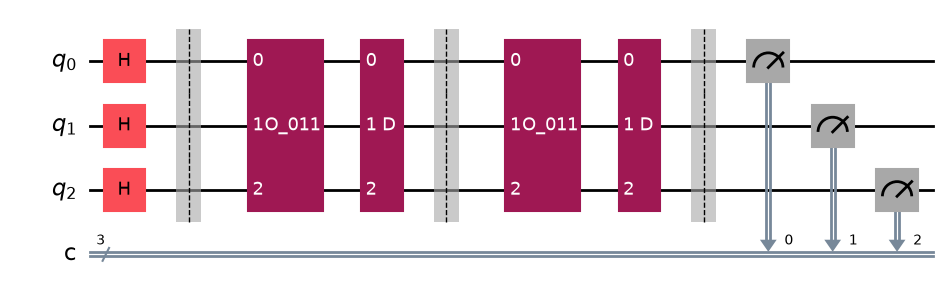
\includegraphics[width=0.8\textwidth]{imagenes/bloque4/e4_2_circuito_minimoK.png}
    \caption{Algoritmo de Grover para $N=8$ y $w=011$ con $k=2$ iteraciones. Cada iteración está formada por el oráculo $O$ y el operador de difusión $D$.}\label{fig:bloque4_e4_2_circuito}
\end{figure}

\textbf{Predicción.} Tras $k=2$ iteraciones, el estado marcado se mide con probabilidad $P_2=0{,}9453$ y cada uno de los otros siete estados con probabilidad $(1-P_2)/7=0{,}0078$. En 4096 disparos se esperan $3872$ conteos para $|011\rangle$ y $32$ para cada uno de los demás.
La comparación con la simulación se muestra en la Tabla~\ref{tab:bloque4_e4_2_hist} y en la Figura~\ref{fig:bloque4_e4_2_hist}.

\begin{table}[htbp]
    \centering
    \begin{tabular}{c|c|c|c|c}
    \hline
    Estado & $P$ teórica & $P$ simulada & Conteo teórico & Conteo simulado \\
    \hline
    \texttt{000} & 0,0078 & 0,0066 & 32 & 27 \\
    \texttt{001} & 0,0078 & 0,0081 & 32 & 33 \\
    \texttt{010} & 0,0078 & 0,0073 & 32 & 30 \\
    \texttt{011} & 0,9453 & 0,9475 & 3872 & 3881 \\
    \texttt{100} & 0,0078 & 0,0071 & 32 & 29 \\
    \texttt{101} & 0,0078 & 0,0100 & 32 & 41 \\
    \texttt{110} & 0,0078 & 0,0066 & 32 & 27 \\
    \texttt{111} & 0,0078 & 0,0068 & 32 & 28 \\
    \hline
    \end{tabular}
    \caption{Ejercicio 4.2: probabilidades y conteos teóricos y simulados con $k=2$ (4096 disparos).}\label{tab:bloque4_e4_2_hist}
\end{table}

\begin{figure}[h]
    \centering
    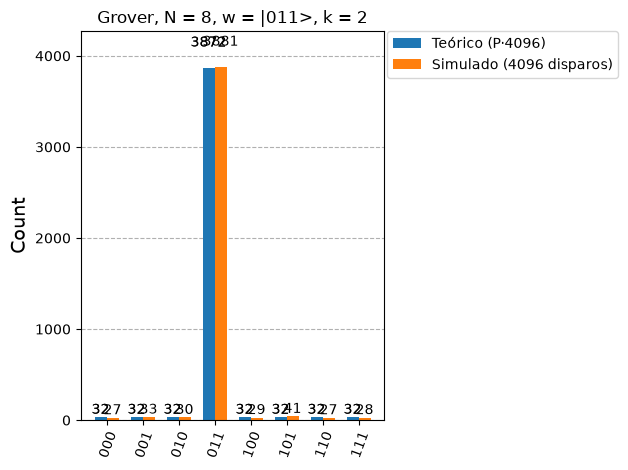
\includegraphics[width=0.5\textwidth]{imagenes/bloque4/e4_2_histograma_comparacion.png}
    \caption{Comparación del histograma simulado (4096 disparos) con la predicción teórica para $N=8$, $w=|011\rangle$ y $k=2$.}\label{fig:bloque4_e4_2_hist}
\end{figure}

\textbf{Resultado.} El histograma simulado reproduce la predicción: el estado marcado se mide con probabilidad 
$0{,}9475$ frente al valor teórico $0{,}9453$, y los siete restantes aparecen con frecuencias del orden de $0{,}7\%$.
El test $\chi^2$ de bondad de ajuste da un $p$-valor de $0{,}654$, compatible con la teoría al $5\%$.

%--------------------------------------------------------------------
\subsection{Ejercicio 4.3. Límite de probabilidad}
La probabilidad de éxito es $P_k(w)=\sin^2((2k+1)\theta)$, que solo vale 1 si $(2k+1)\theta=\pi/2+m\pi$ para algún entero $m$. Con $\theta=0{,}36137$ rad,
$$(2k+1)\theta=\frac{\pi}{2}\;\Longrightarrow\;k=\frac{1}{2}\Big(\frac{\pi}{2\theta}-1\Big)=1{,}673,$$
que no es un entero. Por tanto, en la \emph{primera} subida de $P_k$ no se alcanza el 1: el mejor entero es $k=2$, con $P_2=0{,}9453<0{,}99$. En esta primera subida \textbf{no es posible} llegar al $99\%$.

Sin embargo, $P_k$ es periódica en $k$ con periodo $\pi/(2\theta)=4{,}347$, que no es un entero, de modo que a medida que crece $k$ los valores $(2k+1)\theta$ recorren puntos distintos de cada ciclo y alguno puede caer muy cerca de $\pi/2+m\pi$.
Se tiene $P_k\ge0{,}99$ si y solo si $|(2k+1)\theta-(\pi/2+m\pi)|\le\arccos(\sqrt{0{,}99})=0{,}100$ rad. Para $k=2$ la diferencia es $0{,}236$ rad (no basta), pero para $\boldsymbol{k=6}$ se obtiene
$$13\,\theta=4{,}6978\ \text{rad}\ \text{frente a}\ \frac{3\pi}{2}=4{,}7124\ \text{rad},$$
es decir, una diferencia de solo $0{,}015$ rad y $P_6=0{,}99979$. La simulación lo confirma ($P_6=0{,}9993$). La Figura~\ref{fig:bloque4_e4_3} muestra $P_k$ frente a $k$ (teórica y simulada) y la Tabla~\ref{tab:bloque4_e4_3} recoge los valores.

\begin{figure}[h]
    \centering
    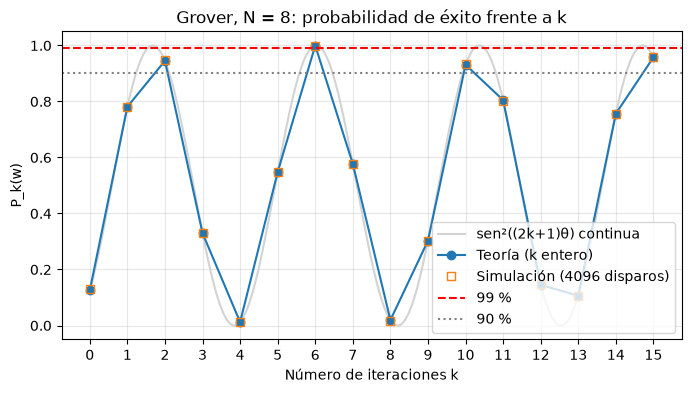
\includegraphics[width=0.8\textwidth]{imagenes/bloque4/e4_3_90percExito.png}
    \caption{Probabilidad de éxito $P_k(w)$ frente al número de iteraciones 
    $k$ para $N=8$: teoría (línea) y simulación con 4096 disparos (cuadrados). Se indican los umbrales del 
    $90\%$ y del $99\%$.}\label{fig:bloque4_e4_3}
\end{figure}

\begin{table}[htbp]
    \centering
    \begin{tabular}{c|c|c|c||c|c|c|c}
    \hline
    $k$ & $(2k+1)\theta$ & teórica & simulada & $k$ & $(2k+1)\theta$ & teórica & simulada \\
    \hline
    0 & 0,3614 & 0,1250 & 0,1313 & 8  & 6,1432  & 0,0195 & 0,0171 \\
    1 & 1,0841 & 0,7813 & 0,7795 & 9  & 6,8660  & 0,3029 & 0,3022 \\
    2 & 1,8068 & 0,9453 & 0,9475 & 10 & 7,5887  & 0,9313 & 0,9343 \\
    3 & 2,5296 & 0,3301 & 0,3318 & 11 & 8,3114  & 0,8049 & 0,8035 \\
    4 & 3,2523 & 0,0122 & 0,0115 & 12 & 9,0342  & 0,1450 & 0,1475 \\
    5 & 3,9750 & 0,5480 & 0,5483 & 13 & 9,7569  & 0,1063 & 0,1057 \\
    6 & 4,6978 & 0,9998 & 0,9993 & 14 & 10,4796 & 0,7566 & 0,7568 \\
    7 & 5,4205 & 0,5770 & 0,5784 & 15 & 11,2024 & 0,9578 & 0,9583 \\
    \hline
    \end{tabular}
    \caption{Ejercicio 4.3: probabilidad de éxito de Grover para $N=8$ y $k=0,\dots,15$.}\label{tab:bloque4_e4_3}
\end{table}

\textbf{Resultado.} Con $N=8$ el máximo de la primera subida es el $94{,}5\%$ ($k=2$), y ese es el límite si solo se consideran los primeros valores de $k$. Pero la probabilidad no está acotada por ese valor: como el periodo de $P_k$ no es entero,
sí es posible superar el $99\%$, y el primer $k$ que lo consigue es $k=6$ ($99{,}98\%$ teórico, $99{,}93\%$ simulado). En el rango estudiado ($k\le15$) es el único. Hay que tener en cuenta el coste: $k=6$ iteraciones implican 6 consultas al oráculo, más que las $\approx N/2=4$
consultas de media del algoritmo clásico, de modo que para un $N$ tan pequeño la ventaja cuadrática de Grover no se manifiesta; además, el resultado es muy sensible a $k$ ($P_5=0{,}548$ y $P_7=0{,}577$).